
\documentclass[./thesis.tex]{subfiles}

 
\begin{document}


\alert{ Il faut ecrire quelque part la fonction d'onde:
$$ \ket{\Psi} = \sum_I^\Ndet c_I \kI $$
et l'expression des determinants:
\begin{equation}
\begin{array}{c}
 \Psi({\bf r}_1,\dots,{\bf r}_{\Na},{\bf r}_{\Na+1},\dots,{\bf r}_N;
      \alpha_1,\dots,\alpha_{\Na},\beta_{\Na+1},\dots,\beta_N) = \\
\left|
 \begin{array}{ccc}
 \varphi_1({\bf r}_1) & \dots & \varphi_1({\bf r}_{\Na}) \\
 \vdots               & \dots &   \vdots             \\
 \varphi_{\Na}({\bf r}_1) & \dots & \varphi_{\Na}({\bf r}_{\Na}) \\
 \end{array}
\right|
\left|
 \begin{array}{ccc}
 \varphi_1({\bf r}_{\Na+1}) & \dots & \varphi_1({\bf r}_{N}) \\
 \vdots               & \dots &   \vdots             \\
 \varphi_{N_\beta}({\bf r}_{\Na+1}) & \dots & \varphi_{N_\beta}({\bf r}_{N}) \\
 \end{array}
\right|
\end{array} 
\label{eq:slater}
\end{equation}
}

Generally speaking, implementing a wavefunction method requires iteration over either two-electron integrals or determinants. \\
ease of implementation VS performances \\
ease of parallelism(?) \\
Need to explicitly maintain a list of determinant. \\




\section{Notation TBUpdated}
\begin{itemize}
	\item [$\Ne$] : Number of electrons.
	\item [$\Na$] : Number of $\alpha$-spin electrons.
	\item [$\Nb$] : Number of $\beta$-spin electrons.
	\item [$\Ndet$] : Number of determinants in the wavefunction.
	
	\item [$\Norb$] : Number of orbitals.

	\item [$\Nint$] : Number of 64-bit integers required to store $\Norb$ bits.
        $\Nint = \lfloor \frac{\Norb-1}{64} \rfloor + 1$
		
	\item [$\bitI$] : Bitstring representation of $\kI$
\begin{lstlisting}
integer*8 :: I(N_int, 2)
\end{lstlisting}
	
	\item [$\bitIsigma$] : 
	Bitstring representation of $\sigma$ spinorbitals of $\kI$, $\sigma \in \{\alpha, \beta\}$ 
\begin{lstlisting}
integer*8 :: Is(N_int)
\end{lstlisting}

	\item [ {$\bitIsigma [n] $} ] :
	Bitstring representation of $\sigma$ spinorbitals of $\kI$ in the range $[ 1+n \times 64, \min \qty (n \times 64 + 63, \Norb) ]$, $0 \leq n \leq \Nint-1 \; ;\; \sigma \in \{\alpha, \beta\}$
\begin{lstlisting}
integer*8 :: Isn
\end{lstlisting}

\end{itemize}

All the program is built such that the $\alpha$ and $\beta$ spinorbitals share the same space part. In other words, spinorbitals $i$ and $\bar{i}$ both refer to orbital $\phi_i(\br)$.


\section{Determinant internal representation}
\label{sec:det_representation}

Determinants can be written as a string of creation operators applying to the vacuum state $\vac$.
\begin{equation}
\ac{i} \ac{j} \ac{k} \vac = \kI
\end{equation}
Because of the fermionic nature of electrons, permutation of two contiguous creation operators results in a sign change, which makes their ordering relevant.
\begin{align}
\ac{j} \ac{i} & = -\ac{i} \ac{j} \\
\ac{j} \ac{i} \ac{k} \vac &=  -\kI
\end{align}
This effectively allows to make any $\Nperm$ permutations (even of non-contiguous operators), and always get $-1^{\Nperm} \kI.$

We see a determinant can be broken down into two pieces of information:
\begin{itemize}
\item
A set of creation operators, corresponding to the set of occupied spinorbitals in the determinant.
\item
An ordering of the creation operators, responsible for the sign of the determinant. Once a common ordering operator $\ordering$ is chosen, it is sufficient to store the sign change that will occur when this operator is applied to the string of creation operators. This sign will be referred to as the \emph{phase factor}.
\end{itemize}
Determinants are always associated with a coefficient, so
if the determinants are always built after applying them the same common ordering operator,
we don't need to make the phase factor part of the determinant's internal representation. The sign may simply be reported on the associated coefficient.

In this thesis, all the determinants will be built using the order where all the $\alpha$ spinorbitals are placed before the $\beta$ spinorbitals:
\begin{equation}
\label{eq:spinpack}
\ordering \kI = \hat{I} \vac = \hat{I}_\alpha \hat{I}_\beta \vac 
\end{equation}
and within each operator $\hat{I}_\alpha$ and $\hat{I}_\beta$, the creation operators are sorted with increasing indices.
For instance, consider the determinant built from the set of spinorbitals $\{i,j,k,{\bar i} \}$ with $i<j<k$,
\begin{equation}
\kJ = \ac{j} \ac{k} \ac{\bar i} \ac{i} \vac.
\end{equation}
If we happen to encounter such a determinant, our choice of representation imposes us to consider its re-ordered expression
\begin{equation}
\ordering \kJ = - \ac{i} \ac{j} \ac{k} \ac{\bar i} \vac 
\end{equation}
and the sign change (or \emph{phase factor}) will need to be handled.

The indices of the creation operators (or equivalently the
occupations of the spinorbitals), are stored using the so-called \emph{bitstring} encoding. A bitstring is an array of bits ; typically, the 64-bit binary representation of an integer is a bitstring of size 64.
Quite simply, the idea is to map each spinorbital to a single bit, whose value is set to its occupation number. In other words \texttt{0} and \texttt{1} are associated with the \emph{unoccupied} and \emph{occupied} states.
By this definition, bitstrings are essentially lists of occupation numbers, which is a convenient way to
store the set of occupied spinorbitals in a determinant, with the predefined ordering.

For simplicity and performance considerations, the occupations of the $\alpha$ and $\beta$ spinorbitals are stored on different bitstrings, rather than interleaved or otherwise merged in the same one. This allows to straightforwardly map orbital index $n$ to bit index $n-1$ (orbitals are usually indexed from $1$, while bits are indexed from $0$), and makes a bitstring a set of orbitals.
This makes the representation of a determinant a tuple of two bitstrings, associated with respectively $\alpha$ and $\beta$ spinorbitals. Such objects are refered to as \emph{$\alpha \beta$-bitstrings}, and generally define a set of spinorbitals. When used to define a determinant, they imply the previously defined ordering.


\begin{itemize}
\item
$\bitI$ is the $\alpha \beta$-bitstring representation of $\kI$
\item
$\bitI_\alpha$ is the bitstring representation of the set of occupied $\alpha$ spinorbitals of $\kI$ 
\item
$\bitI_\beta$ is the bitstring representation of the set of occupied $\beta$ spinorbitals of $\kI$ 

\end{itemize}


The storage space required for a single determinant is, in principle, one bit per spinorbital, or $2 \times \Norb$ bits. However, because CPUs are designed to handle efficiently 64-bit integers, each spin part is stored as an array of 64-bit integers, the unused space being padded with zeros. 
The actual storage needed for a determinant is $2 \times 64 \times \Nint$ bits, where $\Nint$ is the number of 64-bits integers needed to store one spin part:
\begin{equation}
\Nint = \left \lfloor \frac{\Norb-1}{64} \right \rfloor + 1.
\end{equation}


The Fortran representation of a bitstring is an array of $\Nint$ \lstinline{integer*8}'s (64-bit integers).  
The Fortran representation of an $\alpha \beta$-bitstring is a two dimensional array of \lstinline{integer*8}'s, the first dimension of size $\Nint$ and the second of size $2$, corresponding to the $\alpha$ and $\beta$ spin parts.


\lstset{frame=single}
\begin{lstlisting}
  ! I is an ab-bitstring
  ! I_alpha and I_beta are bitstrings
  
  integer*8 :: I(N_int, 2)
  integer*8 :: I_alpha(N_int), I_beta(N_int)

  ... ! load some determinant in I
  I_alpha(:) = I(:,1)
  I_beta (:) = I(:,2)
\end{lstlisting}
\lstset{frame=none}


In formulas or algorithms, depending on the level of detail desired, a bitstring may also be treated as a single mathematical integer (in $\mathbb{Z}$), avoiding the cumbersome separation into 64-bit packs. However, in algorithms we will usually try to stay closer to the actual implementation. $\bitI$ being the $\alpha \beta$-bitstring associated with $\kI$, we can explicitly refer to a single element of the 64-bit integer array as
\begin{equation}
\bitI_{\sigma}[i]\; ;\; \sigma \in \{\alpha, \beta\}\; ;\; i \in [0, \Nint[
\end{equation}
which is the bitstring representation of the $\sigma$ spinorbitals of determinant $\kI$ in the range $[1+i \times 64, \min \left( (i+1) \times 64, \Norb \right)]$, indexed from $0$ to $63$.

      
\section{Bit manipulation}

The bitstring encoding is a compact way of storing determinants, but it is more than just a storage method. It allows to perform a variety of operations on determinants by taking advantage of CPU's hardware aptitude to perform efficiently bitwise operations on integers.

In many of the presented algorithms, some Fortran intrinsics will be of use. Each of those maps to a CPU instruction that is available on modern CPUs.


\begin{sloppypar}
\begin{itemize}
	      
	\item $\POPCNT{\bitI}$ :
	Returns the number of non-zero bits for a given integer $\bitI$. \\
        ${\POPCNT{\binary{00011000}} = 2}$.
	      
	\item $\TRAILZ{\bitI}$ : Returns the number of trailing zero bits for a given integer \bitI. \\
         ${\TRAILZ{\binary{00000100}} = 2}$.
	      
	      
	\item $\IBCLR{\bitI}{n}$ : Returns the value of $\bitI$ with the bit at the $n$-th position set to zero (the rightmost bit is at position zero). \\
        ${\IBCLR{\binary{00001111}}{2} = \binary{00001011}}$.
	      
	     
   	\item $\IOR{\bitI}{\bitJ}$ : Bitwise \texttt{OR} logical operation. \\
        ${\IOR{\binary{1100}}{\binary{1010}} = \binary{1110}}$.

	 
	\item $\IEOR{\bitI}{\bitJ}$ : Bitwise \texttt{XOR} (exclusive or) logical operation. \\
        ${\IEOR{\binary{1100}}{\binary{1010}} = \binary{0110}}$.
	      
	      
	\item $\IAND{\bitI}{\bitJ}$ : Bitwise \texttt{AND} logical operation. \\
        ${\IAND{\binary{1100}}{\binary{1010}} = \binary{1000}}$.
	      
	      
	\item $\NOT{\bitI}$ : Bitwise \texttt{NOT} logical operation. \\
        ${\NOT{\binary{00001100}} = \binary{11110011}}$.
	      
	\item $\ISHFT{\bitI}{n}$ : Returns $\bitI$ with bits shifted $|n|$ places to the left if $n>0$, otherwise to right. Bits shifted out of the range are lost. Zeros are shifted from the opposite end. \\
        ${\ISHFT{\binary{01001110}}{2} = \binary{00111000}}$, \\
        ${\ISHFT{\binary{01001110}}{-2} = \binary{00010011}}$.
	      
	\item $\BTEST{\bitI}{n}$ : Returns $\TRUE$ if the $n$-th bit of $\bitI$ is set, otherwise $\FALSE$. \\
        $\BTEST{\binary{00001000}}{3} = \TRUE$.
	      
\end{itemize}
\end{sloppypar}
      
      
Those intrinsics apply to integers at most 64-bits. This however is a purely implementational limitation, so depending on the level of detail desired, this constraint can be unambiguously lifted in formulas or algorithms. Different notations will be used for the 64-bit and the infinite size cases, as they are not always equivalent.
For example, the $\ISHFT{\_}{\_}$ Fortran intrinsic always returns zero for shifts greater than 64 bits, which is not the case for the $\ishft{\_}{\_}$ function over mathematical integers.
So it is convenient to introduce functions and notations acting on mathematical integers. All binary operators are of same precedence and left-associative.

\begin{table}[H]
	\begin{tabularx}{\textwidth}{X|X}
		\hline
		
		\hline
		\rule{0pt}{3ex}
		$\ISHFT{\bitI}{n}$ & $\ishft{I}{n}$  \\ 
		
		\hline
		\rule{0pt}{3ex}
		$\TRAILZ{\bitI}$ & $\trailz{I}$  \\ 
		
		\hline
		\rule{0pt}{3ex}
		$\IBCLR{\bitI}{n}$ & $\ibclr{I}{n}$  \\ 
		
		\hline
		\rule{0pt}{3ex}
		$\BTEST{\bitI}{n}$ & $\btest{I}{n}$  \\ 
		
		\hline
		\rule{0pt}{3ex}
		$\NOT{\bitI}$ & $\neg I $  \\ 
		
		\hline
		\rule{0pt}{3ex}
		$\IAND{\bitI}{\bitJ}$ & $\iand{I}{J}$ \\
		
		\hline
		\rule{0pt}{3ex}
		$\IOR{\bitI}{\bitJ}$ & $\ior{I}{J}$ \\
		
		\hline
		\rule{0pt}{3ex}
		$\IEOR{\bitI}{\bitJ}$ & $\ieor{I}{J}$ \\
		
		\hline
		\rule{0pt}{3ex}
		$\POPCNT{\bitI}$ & $\popcnt{I}$ \\
		\hline
	\end{tabularx}
\end{table}


Some examples of how these instructions can be used are given below. They are key to understand how we can determine the holes and particles involved in the $\excdet{I}{J}$ excitation operator defined as
\begin{equation}
\excdet{I}{J} \kI = \kJ.
\end{equation}
Let $\bitI$ and $\bitJ$ be the bitstring representations of $\kI$ and $\kJ$, and $\bit{P}$ a bitstring with $\Nint=1$. 


\begin{itemize}
	      
	\item $I_{\alpha}$ : bitstring representation of the set of $\alpha$ spinorbitals of $\kI$
	            
	\item $\popcnt{I_{\alpha}}$ : number of spinorbitals in $I_{\alpha}$ (equal to the number of $\alpha$ electrons).
	            
	\item $\ieor{I_{\alpha}}{J_{\alpha}}$ : bitstring representation of the set of $\alpha$ spinorbitals that are present in either $I_{\alpha}$ or $J_{\alpha}$, but not in both (exclusive disjunction).
        This operator identifies the $\alpha$ spinorbitals involved in the excitation from $\kI$ to $\kJ$. 
	            
	\item $\iand{I_{\alpha}}{\qty(\ieor{I_{\alpha}}{J_{\alpha}})}$ : 
        bitstring representation of the set of $\alpha$ spinorbitals of $\kI$ involved in the excitation from $\kI$ to $\kJ$. This corresponds to the indices of the holes in the excitation $\excdet{I}{J}$ or to the particles in $\excdet{J}{I}$. 
	            
	\item $\popcnt{\ieor{I_{\alpha}}{J_{\alpha}}}/2$ : because the excitation of an electron involves 2 spinorbitals (one hole and one particle), this is the $\alpha$ excitation degree between $\kI$ and $\kJ$.
	            
	\item $\trailz{\bit{P}}+1$ : the index of the lowest orbital in $\bit{P}$. If $\bit{P}$ is $0$, returns $65$.
	            
	\item $\IBCLR{\bit{P}}{\TRAILZ{\bit{P}}}$ : $\bit{P}$ without its orbital of lowest index.

\end{itemize}


\section{Computing Excitations}

An algorithm used to compute the excitation degree is presented as algorithm \ref{alg:EXC_DEGREE}, and one to compute the sets of created holes and particles as algorithm \ref{alg:EXC}. Algorithm \ref{alg:EXC}, however, returns the sets as bitstrings. Extracting the indices from a bitstring is another basic operation, presented as algorithm \ref{alg:LIST_FROM_BITSTRING}.
Because computing excitations is a hotspot of the program, and because we are typically interested in double excitations at most, a more specialized algorithm can be used (\alert{PAS ENCORE ECRIT/POMPÉ}).


\begin{algorithm}[h!]
	\caption{EXC\_DEGREE}
	\label{alg:EXC_DEGREE}
	\SetKwFunction{FMain}{EXC\_DEGREE}
	\SetKwProg{Fn}{Function}{:}{}
	
	\Fn(\tcc*[h]{Computes the excitation degree between two determinants}){\FMain{$I, J$}}{
		\KwData {$I, J$ bitstring representations of determinants $\kI$ and $\kJ$}
		\KwResult{ Returns the excitation degree between $\kI$ and $\kJ$ }

		$X \gets 0$   \;
		\For{$\sigma \in \{\alpha, \beta\}$}{
		\For{$i \gets 0,  \Nint-1$}{
		  $X \gets X+\POPCNT{\IEOR{I_{\sigma}[i]}{J_{\sigma}[i]}}$  \;
		}
		}
		\KwRet $X / 2$\;
	}
\end{algorithm}


\begin{algorithm}[H]
	\caption{EXC}
		
	\SetKwFunction{FMain}{EXC}
	\label{alg:EXC}
	\SetKwProg{Fn}{Function}{:}{}
	
	\Fn(\tcc*[h]{Returns the holes and particles created in an excitation, as bitstrings}){\FMain{$I$,$J$}}{
	\KwData{ $I$ and $J$, the bitstring representations of determinants $\kI$ and $\kJ = \excdet{I}{J} \kI$}
	\KwResult{ Returns a tuple $(P,H)$, where $P$ and $H$ are respectively the sets of particles and holes created by $\excdet{I}{j}$, as $\alpha \beta$-bitstrings}
		\For{$\sigma \in \{\alpha, \beta\}$}{
		\For{$i \gets 0, \Nint-1$}{
			$C \gets \IEOR{I_{\sigma}[i], J_{\sigma}[i]}$\;
			$P_{\sigma}[i] \gets \IAND{C, J_{\sigma}[i]}$\;
			$H_{\sigma}[i] \gets \IAND{C, I_{\sigma}[i]}$\;
		}
		}
		\KwRet{ $(P,H)$}\;
		}
\end{algorithm}




\begin{algorithm}[h!]
	\caption{LIST\_FROM\_BITSTRING}
	\label{alg:LIST_FROM_BITSTRING}
	\SetKwFunction{FMain}{LIST\_FROM\_BITSTRING}
	\SetKwProg{Fn}{Function}{:}{}
	
	\Fn(\tcc*[h]{Returns the indices contained in a bitstring as a list of integers}){\FMain{$P$}}{
		\KwData{ $P$ a bitstring }
		\KwResult{ $L$ the list of indices of the bits set in $P$ in increasing order. $P$ is destroyed. }
		$k \gets 0$ \;
		\For{$i \gets 0, \Nint-1$}{
		\While{$P[i] \neq 0$}{
		$e \gets \TRAILZ{P[i]}$\;
		$P[i] \gets \IBCLR{P[i]}{e}$\;
		$L[k] \gets e + i \times 64$\;
                $k \gets k+1$\;
		}
		\KwRet{$L$}
		}
		}
		
\end{algorithm}



\section{Computing phase factors}


The computation of phase factors is slightly more complex. The following explanation is limited to one spin part. More detail will be given later about why spin parts can be treated independently.
As we have seen in section~\ref{sec:det_representation}, the $\alpha \beta$-bitstring representation of determinants implies an ordering of creation operators : first all the $\alpha$ operators, then all the $\beta$, both with increasing orbital indices.

Whenever we build a new determinant by applying an excitation operator, we obtain a determinant that is initially expressed not just with a different ordering, but with a mix of creation and annihilation operators.

First of all, we have to make this initial expression unambiguous by precisely defining excitation operators. We have defined an implicit ordering for the expression of determinants, we also need an implicit ordering for the expression of excitation operators.
Like for determinants, we pack together $\alpha$ and $\beta$ operators.
\begin{equation}
\label{eq:spinpackexc}
\hat T = \hat T_\alpha \hat T_\beta.
\end{equation}
Within $\hat T_\alpha$ and $\hat T_\beta$, the creation and annihilation operators are separately sorted with increasing indices, then interleaved starting with a creation. In other words, $\hat T_\alpha$ and $\hat T_\beta$ are written as a products of single excitations, lowest particle with lowest hole, then second lowest particle with second lowest hole, \textit{etc}, and we arbitrarily chose to put creation before annihilation operators.
For example, the double excitation $\excorb{ab}{cd}$ with $a<b<c<d$ is expressed as
\begin{equation}
\hat T_{ab}^{cd} = \ac{c} \an{a} \ac{d} \an{b} = \hat T_a^c \hat T_b^d.
\end{equation}

We now can express $\hat T \kI$ as a series of operators.
In most cases, permuting contiguous operators will still just result in a sign change.
\begin{align}
\an{j} \an{i} & = -\an{i} \an{j} \\
\ac{j} \an{i} & =
  \begin{cases}
  -\an{i} \ac{j} & i \ne j \\
  1 - \an{i} \ac{i} & i = j.
  \end{cases}
\end{align}
A particular case is the permutation of a creation and an annihilation operator with the same index.
Indeed, if spinorbital $l$ is unoccupied in $\kI$,
\begin{align}
\label{eq:aa+}
\an{l} \ac{l} \kI & = \kI  \\
\ac{l} \an{l} \kI & = 0 .
\end{align}
In the first case, a particle is created then annihilated, resulting in the same determinant. In the second case, there is an attempt at annihilating a particle that does not exist, resulting in $0$. It is of course the opposite if $l$ is occupied in $\kI$.
These formulas will be used to remove annihilation operators from the expression of a determinant.



Let $\kI$ and $\kK$ be two determinants with spin orbitals ordered as in the $\alpha \beta$-bitstring  representation:
\begin{align}
\kI & = \ac{i}\ac{j}\ac{k} \vac \\
\kK & = \ac{i}\ac{k}\ac{l} \vac
\end{align}
with $i<j<k<l$.
When one applies the excitation operator $\excorb{j}{l}$ to $\kI$,
\begin{equation}
\excorb{j}{l} \kI = \ac{l} \an{j} \ac{i} \ac{j} \ac{k} \vac.
\end{equation}
To build the corresponding $\alpha \beta$-bitstring, one needs to
reorder the operators by permuting contiguous operators.
It takes $n=1$ permutation to bring $\an{j}$ behind $\ac{j}$:
\begin{equation}
\excorb{j}{l} \kI = -\ac{l} \ac{i} \an{j} \ac{j} \ac{k} \vac.
\end{equation}
Using equation~\ref{eq:aa+},
\begin{equation}
\excorb{j}{l} \kI = -\ac{l} \ac{i} \ac{k} \vac.
\end{equation}
Then, it takes $n$ permutations to bring $\ac{l}$ to the position formerly occupied by $\ac{j}$, and $x=1$ more permutation to bring it at its final position.
\begin{equation}
\excorb{j}{l} \kI = -\ac{i} \ac{k} \ac{l} \vac = -\kJ.
\end{equation}

The total number of permutations needed is $\Nperm = 2n+x$. The parity of the number or permutations is the parity of $x$. As can be seen, $x$ is the number of occupied spinorbitals with indices in the $]j, l[$ range in $\kI$ (regardless of whether $l>j$ or $l<j$). In our case, there was one occupied spinorbital $k$, so $\Nperm$ is odd and we ended with a negative phase factor.

\begin{figure}[h!]
	\begin{center}
		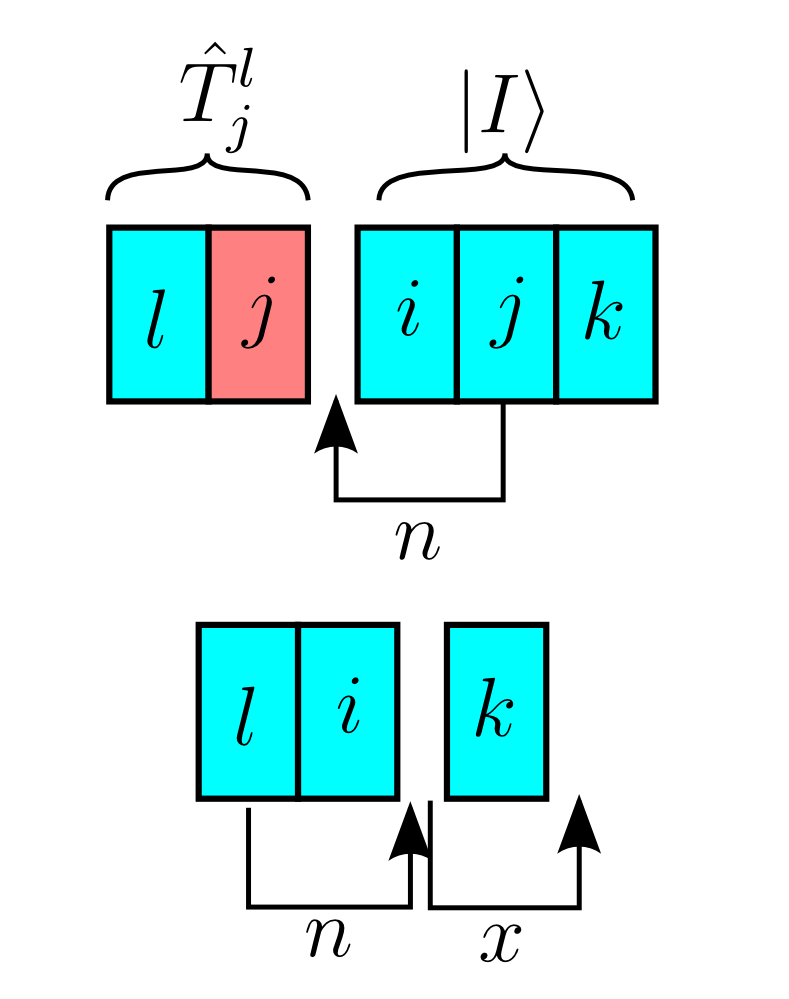
\includegraphics[width=0.3\columnwidth]{figures/determinant_driven/phasefactor}
		\caption{
		\label{phasefactor}%
		\alert{phasefactor}
		}
	\end{center}
\end{figure}

\subsection{Treating spin parts separately}

It is not immediately obvious that $\alpha$ and $\beta$ spin parts can be treated independently. It is possible because our ordering packs together operators of same spin in the expression of both determinants (Eq.\eqref{eq:spinpack}) and excitations (Eq.\eqref{eq:spinpackexc}), and 
also because we never consider excitations where the spin is changed (spin-flips). 
Under these constraints, any excitation operator $\hat{T}$ can be expressed as 
\begin{equation}
\hat{T} = \hat{T}_\alpha \hat{T}_\beta .
\end{equation}

\begin{align}
\label{eq:spin1}
\hat{T} \kI & = \hat{T}_\alpha \hat{T}_\beta \,  \hat{I}_\alpha \hat{I}_\beta \vac \\
\label{eq:spin2}
            & =  \qty(\hat{T}_\alpha \hat{I}_\alpha) \qty(\hat{T}_\beta  \hat{I}_\beta) \vac 
              = \hat{J}_\alpha \hat{J}_\beta  \vac = \kJ.
\end{align}

The number of creation and annihilation operators in an excitation operator is always even. Hence, going from Eq.\eqref{eq:spin1} to Eq.\eqref{eq:spin2} by permuting $\hat{T}_\beta$ with $\hat{I}_\alpha$ always requires an even number of permutations.
So the phase factors can be easily computed by reordering separately $\hat{T}_\alpha \hat{I}_\alpha$ and $\hat{T}_\beta  \hat{I}_\beta$.



\subsection{Single excitations}

%In the case of a monoexcitation, only one spin part is involved. All indices refer to spinorbitals of same, arbitrary spin $\sigma \in \{\alpha, \beta\}$

For a given determinant $\kI$ and a singly excited determinant $\kalpha = \ordering \excorb{i'}{j'} \kI$ where both 
use the ordering of spinorbitals defined previously, the phase factor can be determined by the parity of
\begin{equation}
N^{S}_{ij}=\sum_{k=i+1}^{j-1} \occ{k}{I}
\end{equation}
where $i=\min(i',j')$, $j=\max(i',j')$ and
\begin{equation}
\occ{k}{I} = \delta \qty(\ac{k}\an{k} \kI - \kI) = \begin{cases}
 1 & \text{if } \ac{k}\an{k} \kI = \kI \\
 0 & \text{otherwise}
\end{cases}
\end{equation}
is the occupation number of spinorbital $k$ in determinant $\kI$.\footnote{Note that occupation
numbers in $\kI$ and $\kalpha$ are by construction equal for any spinorbital $k \neq i \neq j$, so while we will use $\kI$ in the following, we could as well use $\kalpha$.
%This is obvious from the fact that $\Hij{I}{\alpha}=\Hij{\alpha}{I}$.
}
We will use the fact that the parity of an integer $X$ can be obtained by extracting the least significant bit of its binary representation: 
\begin{equation}
p(X)=\iand{X}{1} = \begin{cases}
1 & \text{ if $X$ is odd  } \\
0 & \text{ if $X$ is even.} 
\end{cases}.
\end{equation}


A bitstring $R_{ij}$, containing all orbitals in a given range $]i, j[$ can be built as 
\begin{equation}
R_{ij}=\ieor{\ishft{\neg{0}}{i}}{\ishft{\neg{0}}{j-1}}
\end{equation}
where $\neg{0}$ denotes the bitstring where all the bits are set to one.

Let $I$ be the bitstring representation of $\kI$, the number of orbitals of spin $\sigma$ in $\kI$ in the given orbital range can be evaluated as
\begin{equation}
N^{I}_{ij} = \popcnt{\iand{I_{\sigma}}{R_{ij}}}.
\end{equation}
So the phase factor to be applied when going from $\kI$ to $\kalpha$ is 
\begin{equation}
\phase{I}{\alpha} = -1^{p(N^I_{ij})}.
\end{equation}
Using the above formulas and taking into account the bitstring's internal representation as arrays of $\Nint$ \lstinline{integer*8}'s, we get algorithm~\ref{alg:PHASE_MONO}.   


\begin{algorithm}
	\caption{PHASE\_MONO}	
	\label{alg:PHASE_MONO}
				\SetKwFunction{FMain}{PHASE\_MONO}
	\SetKwProg{Fn}{Function}{:}{}
	
	\Fn(\tcc*[h]{Compute phase factor of $\ordering \excorb{a}{b} \kI$}){\FMain{$I_\sigma, a, b$}}{
		\KwData{ $I_\sigma$ the bitstring representation of $\sigma \in \{\alpha, \beta\}$ spinorbitals of $\ket I$}
		\KwData{ $a,b$ indices of a hole and a particle created in $\sigma$ spinorbitals of $\ket I$ }
		\KwResult{ The phase factor associated with $\ordering \excorb{a}{b} \kI$}
		$\texttt{high} \gets \max(a,b)-1$ \;
		$\texttt{low} \gets \min(a,b)-1$ \;
		$il \gets \frac{\texttt{low}}{64} + 1$ \;
		$ih \gets \frac{\texttt{high}}{64} + 1$ \;
		$l \gets \texttt{low} \mod 64$ \;
		$h \gets \texttt{high} \mod 64$ \; 
		\For{$i \gets il, ih-1$}{
			$\texttt{mask}[i] = \texttt{NOT}(0)$\;		
		}

		%$mask[ih] \gets ISHFT(NOT(0), h-63)$ \;
		%$mask[il] \gets IAND(mask[il], ISHFT(NOT(0), l))$ \;
		
		$\texttt{mask}[ih] \gets \texttt{ISHFT}(\texttt{NOT}(0), h+1)$ \;
		$\texttt{mask}[il] \gets \texttt{IEOR}(\texttt{mask}[il], \texttt{ISHFT}(\texttt{NOT}(0), l))$ \;
		
		
		$\Nperm \gets 0$ \;
		\For{$i \gets il,ih$}{
			$\Nperm \gets \Nperm + \texttt{POPCNT}(\texttt{IAND}(I_{i}, \texttt{mask}[i]))$ \;
		}
                $\texttt{phase}[0:1] = [ 1.0 \;;\; -1.0 ]$ \;
                \KwRet $\texttt{phase}[\texttt{IAND}(\Nperm,1)]$ \;
		}
\end{algorithm}


\subsection{Phasemasks}


Algorithm \ref{alg:PHASE_MONO} is a general one, efficient for computing the phase factor for two arbitrary determinants. However, a phase computation is typically needed every time two determinants are compared, resulting in a vast amount of computational power being consumed. When only this method was used in the quantum package, it was not uncommon to find that a large fraction of the computational time was spent in phase computations.
Advantage can be taken of the fact that, in most cases, the considered determinants aren't actually arbitrary. Usually, the phase computation will be performed repeatedly with the same determinant. For a fairly modest computational price, it is possible to compress the phase information from a particular determinant and make it cheaper to extract. The underlying principle is little more than a cumulative sum. If, for a determinant $\ket{S}$ that is going to be used repeatedly for phase computations, we pre-compute
\begin{equation}
E^S(i) = \sum_{k=1}^{i-1} \occ{k}{S},
\end{equation}
we can access $N^S_{ij}$ for any $i$ and $j>i$ with no need to loop over $k$:
\begin{align}
\tilde N^S_{ij} &= E^S(j) - E^S(i+1) \; ; \; i \neq j \\
N^S_{ij} &= \tilde N^S_{ij} \; ; \; j>i.
\end{align}

Note that $\tilde N^S_{ij}$ is still defined when $j<i$. The reason for this will be made clear later.
This requires to store $E^S$ which is an integer array of size $2 \times (\Norb+1)$. 
%Note that there is a slight waste as $E^S_1 = 0 \forall \ket S$ ( there is always $0$ electrons under the first orbital ) and $E^S_{\Norb+1} = N_{electron,\sigma} \forall \ket S$ ( there is always $N_{electron,\sigma}$ electrons in all orbitals ). Those values are still stored for convenience.




%\begin{comment}
%This requires to store $E^S$ which is an integer array of size $2 \times (\Norb+1)$.
%Note that although only $2 \times \Norb$ integers are required to store the whole information, for practical reasons the actual size of the array is $2 \times (\Norb+1)$ because when the last orbital is involved, we need to access $E_{\Norb+1}$. The reason for this loss is that $E_1$ contains no information - there are always 0 electrons under the first orbital, $E^S_1 = 0 \forall \ket S$.
%\end{comment}

This may be somewhat memory consuming if we want to pre-compute and store $E$ for each determinant. However, because the actual information needed isn't $N^S_{ij}$, but merely its parity, we only need to store the so-called ``phasemask'' array $P^S$
\begin{equation}
\label{eq:phasemask}
P^S(i) = p(E^S(i))
\end{equation}
which is 1 bit of information per spinorbital, as opposed to an integer big enough to accommodate a number of electrons.
\begin{align}
E^S(i) & = 2 \times  \lfloor \frac{E^S(i)}{2} \rfloor + P^S(i) \\
\tilde N^S_{ij} & = E^S(j) - E^S(i+1) \\
 & = 2 \times \qty( \lfloor \frac{E^S(j)}{2} \rfloor - \lfloor \frac{E^S(i+1)}{2} \rfloor ) + P^S(j) - P^S(i+1)
\end{align}
	    
In the last equation, $\tilde N^S_{ij}$ is expressed as a sum of 3 terms. The first one being even by construction, the parity of $\tilde N^S_{ij}$ is the parity of the rest of the sum.
\begin{equation}
p(\tilde N^S_{ij})=p(P^S_j - P^S_{i+1})
\end{equation}
This can be rewritten in a slightly more efficient way as
\begin{equation}
p(\tilde N^S_{ij}) = P^S_j \oplus P^S_{i+1}
\end{equation}

%Note that using $E^S$ instead of $P^S$ would require an extra ADD instruction ( totalement negligeable ? )
%\begin{equation}
%p(\tilde N^S_{ij}) = (E^S_{i+1} - E^S_j) \wedge 1
%\end{equation}

We have used sorted indices $i<j$. But just like for the general algorithm, if we consider $\hat T_{i'}^{j'}$ we need to sort $i'$ and $j'$ to get the $i=\min(i', j')$ and $j=\max(i', j')$ indices used for the phase computation.

This however doesn't need to be done explicitly. We can arbitrarily choose $i=i'$ and $j=j'$, and reverse the phase if $j<i$. We effectively have computed $p(N^S_{i'j'})$ instead of $p(N^S_{j'i'})$, and it can be proved they are always of different parity:
\begin{align}
\tilde N^{S}_{i' j'} + \tilde N^{S}_{j'i'} & = E^{S}_{j'} - E^S_{i'+1} + E^S_{i'} - E^S_{j'+1} \\
& = -\qty( \occ{j'}{S} + \occ{i'}{S})
\end{align}
Because $\hat T_{i'}^{j'} \ket S \neq 0$, we know that $\occ{j'}{S} + \occ{i'}{S} = 1$. 
\begin{equation}
\tilde N^{S}_{j' i'} = -(\tilde N^{S}_{i'j'} + 1)
\end{equation}
This translates to $\tilde N^{S}_{j' i'}$ and $\tilde N^{S}_{i'j'}$ being of different parity.

\begin{algorithm}
	\caption{PHASEMASK}	
	\label{alg:PHASEMASK}	
	\SetKwFunction{FMain}{PHASEMASK}
	\SetKwProg{Fn}{Function}{:}{}
	
	\Fn(\tcc*[h]{Compute a phasemask}){\FMain{$I$}}{
		\KwData{ $I$ the bitstring representation of $\ket I$}
		\KwResult{ $P$ is the phasemask vector associated with $\ket I$, as described in Eq.~\eqref{eq:phasemask}}
		   
		\For{$\sigma \in \{\alpha, \beta\}$}{
		 $p \gets 0$ \;
		\For{$i \gets 0, \Nint-1$}{
		 $n \gets \min(64, \Norb - i \times 64)$ \;
		\For{$j \gets 0,n-1$}{
		 $P_\sigma[i \times 64 + j] \gets p$ \;
		\If{$\texttt{BTEST}(I, j)$}{
		 $p \gets \texttt{IEOR}(p, 1)$ \;
		%\Comment flips the first bit
		}
		}
		}
		 $P_\sigma [\Norb] \gets p$ \;
		}
		\KwRet{$P$} \;
		}
\end{algorithm}


\begin{algorithm}
	\caption{PHASEMASK\_bit}	
	\label{alg:PHASEMASK_bit}	
	\SetKwFunction{FMain}{PHASEMASK\_bit}
	\SetKwProg{Fn}{Function}{:}{}
	
	\Fn(\tcc*[h]{Compute a phasemask}){\FMain{$\bitI$}}{
		\KwData{ $\bitI$ the bitstring representation of $\kI$}
		\KwResult{ $\bitP$ is the phasemask vector associated with $\kI$, as described in Eq.~\eqref{eq:phasemask}}
		   
		\For{$\sigma \in \{\alpha, \beta\}$}{
		$r \gets 0$ \;
		\For{$i \gets 0, N_{int}-1$}{
				$\bitPsigma[i] \gets \texttt{IEOR}(\bitIsigma[i], \text{ISHFT}(\bitIsigma[i], 1)$ \;
				$d \gets 2$ \;
				\While{$d < \texttt{bit\_kind\_size}$}{
					$\bitPsigma[i] \gets \text{IEOR}(\bitPsigma[i], \text{ISHFT}(P_\sigma[i], d)$ \;
					$d \gets 2 \times d$ \;
				}
				$\bitPsigma[i] \gets \texttt{IEOR}(\bitPsigma[i], r)$ \;
				\If{$\texttt{IAND}(\texttt{POPCNT}(\bitIsigma[i]), 1) == 1$}{
					$r \gets \texttt{NOT}(r)$ \;			
				}
			}
		}
		\KwRet{$P$} \;
		}
\end{algorithm}



\begin{algorithm}
	\caption{PHASE\_FROM\_PHASEMASK}	
	\label{alg:PHASE_FROM_PHASEMASK}	
	\SetKwFunction{FMain}{PHASE\_FROM\_PHASEMASK}
	\SetKwProg{Fn}{Function}{:}{}
	
	\Fn(\tcc*[h]{Compute phase from phasemask}){\FMain{$P^I$, $i$, $j$}}{
		\KwData{ $P^I$ is the phasemask vector associated with $\kI$, as described in Eq.~\eqref{eq:phasemask}. $i$ and $j$ spinorbitals of spin $\sigma \in \{\alpha, \beta \}$ so that $\excorb{i}{j} \kI \neq 0 $.}
		\KwResult{ The phase factor associated with $\ordering \excorb{i}{j} \kI$.}

		\uIf{$j < i$}{
			$c \gets 1$ \;
		}
		\Else{
			$c \gets 0$ \;		
		}
		\uIf{$\qty(c \oplus P^I_\sigma[i+1] \oplus P^I_\sigma[j]) = 1$}{
		\KwRet{ $-1$}\;}
                \Else{\KwRet{ $1$} \; }
		}
\end{algorithm}


%TODO : J'en suis ici.

                
\begin{figure}[h!]
	\begin{center}
		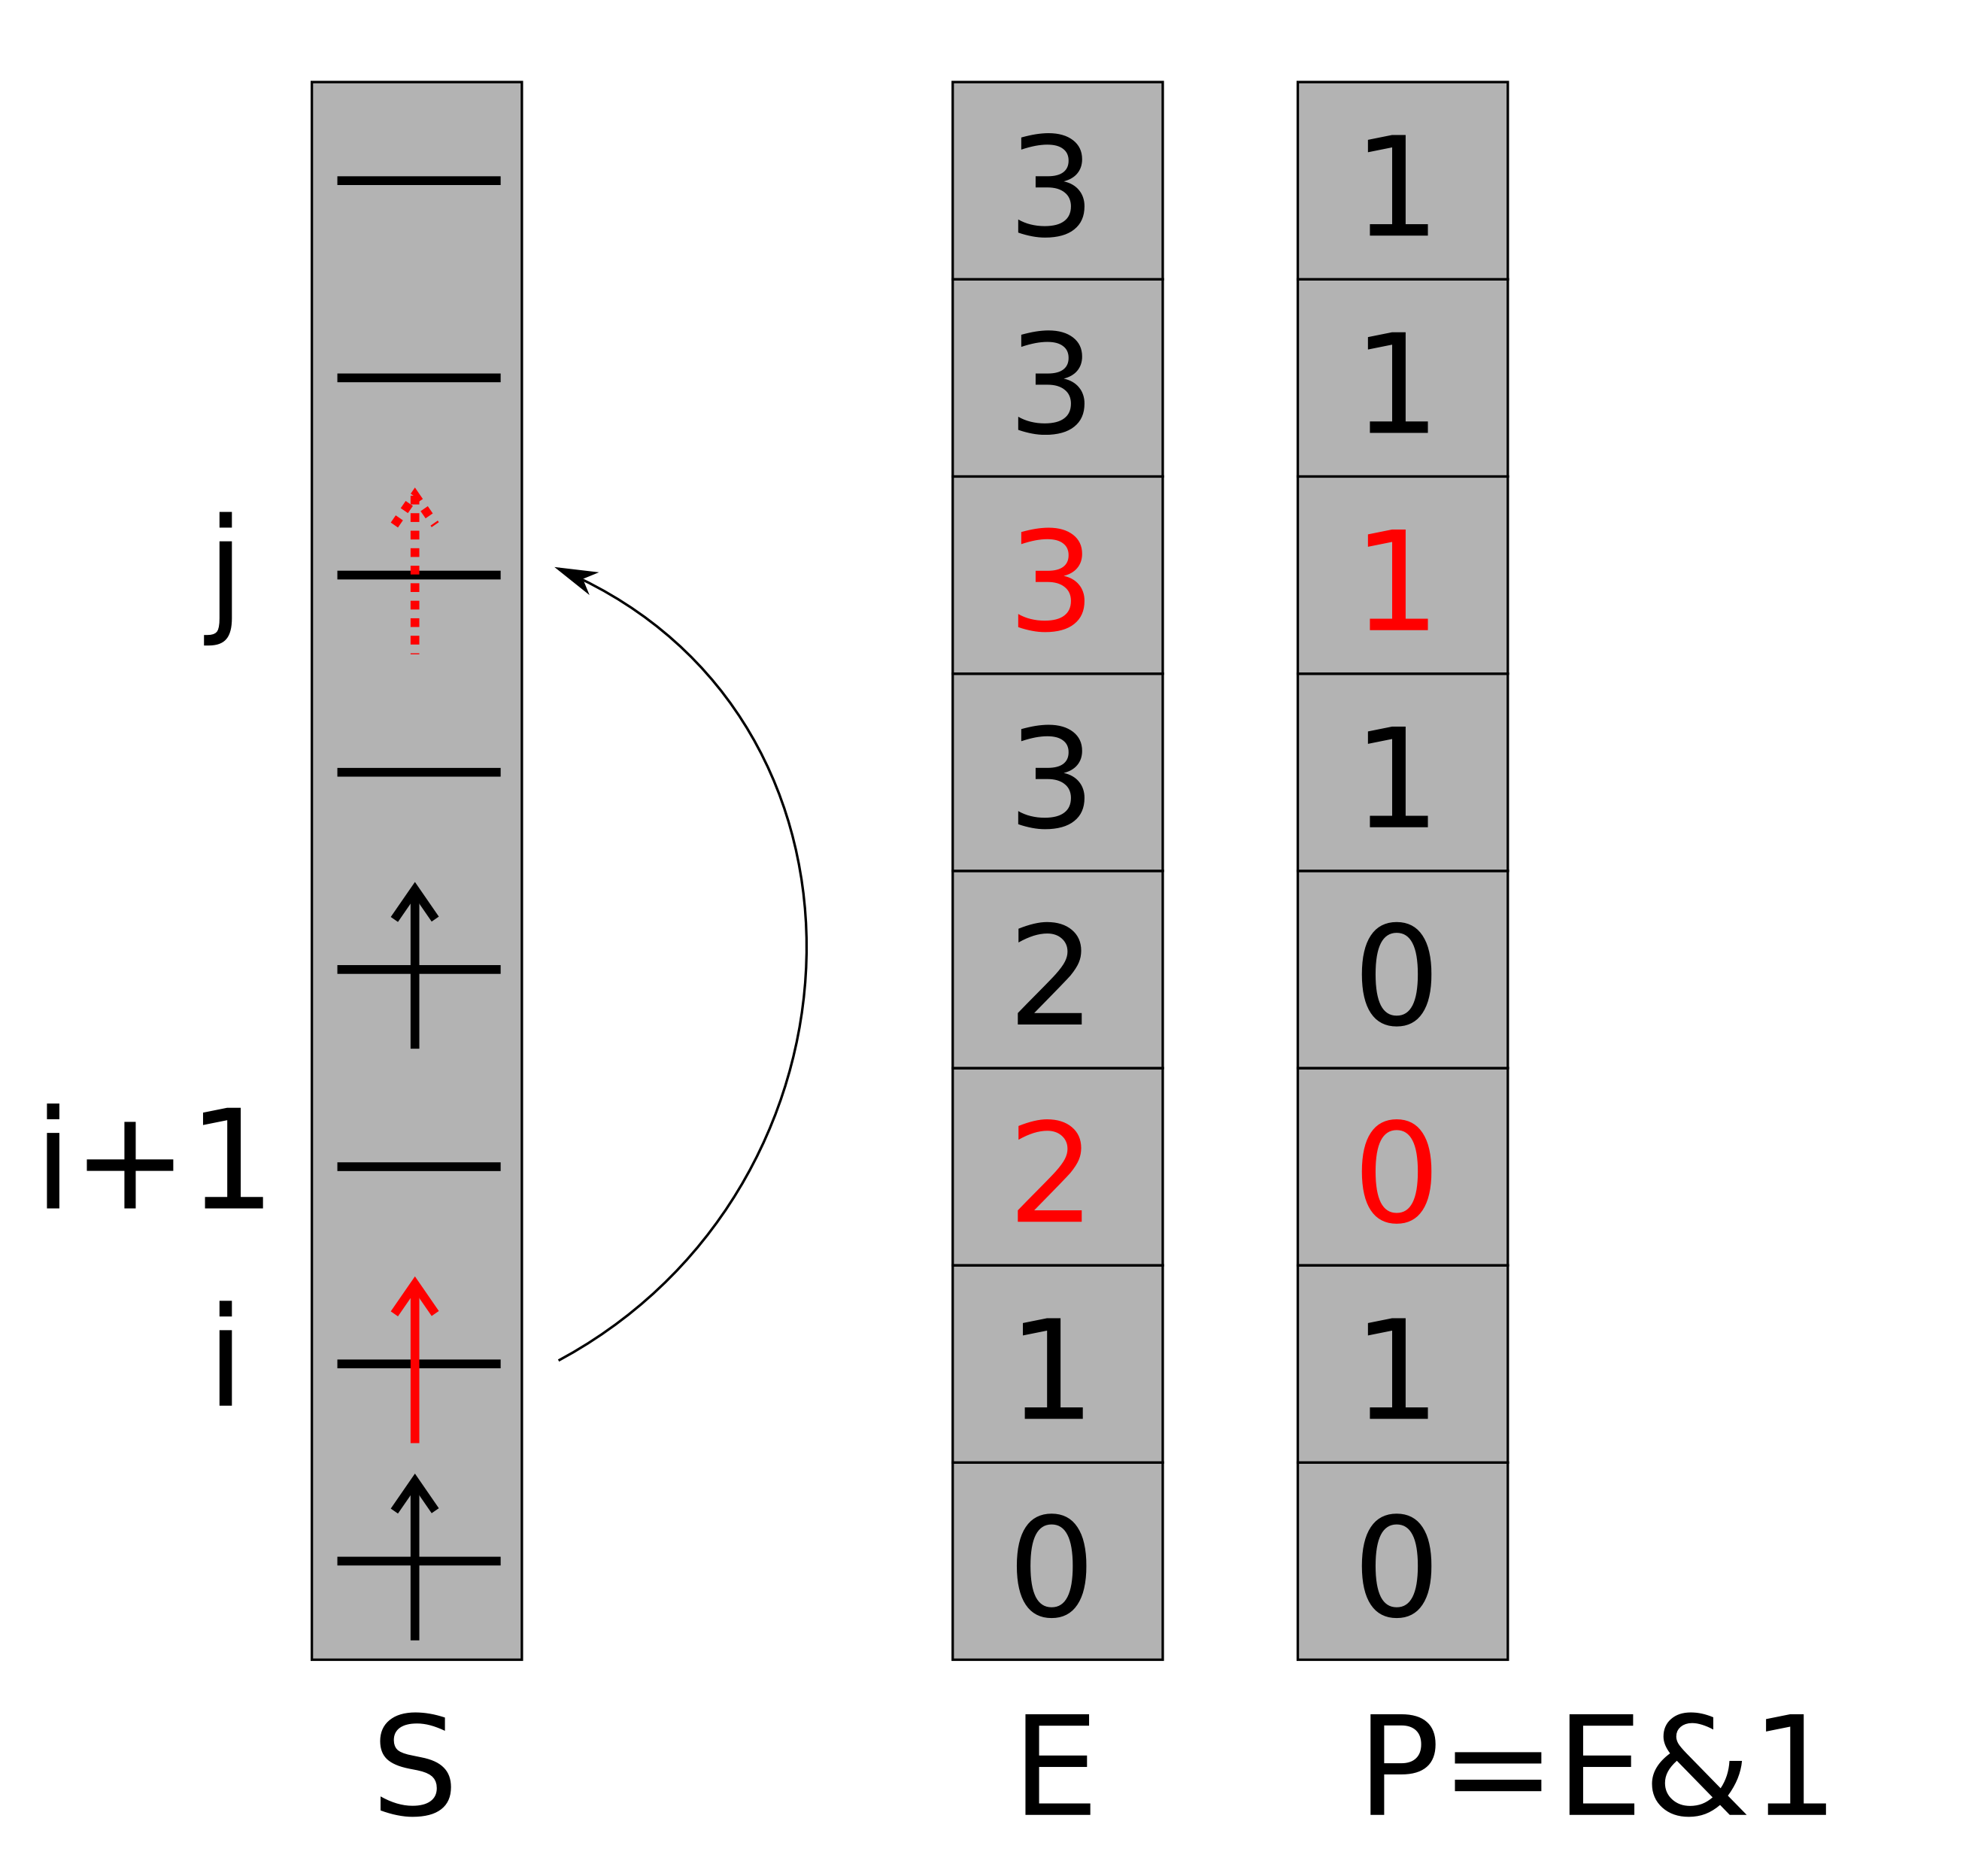
\includegraphics[width=0.6\columnwidth]{figures/determinant_driven/phase}
		\caption{
		\label{generators_selectors}%
		phasemask
		}
		commentt
	\end{center}
\end{figure}
        
Currently, the quantum package does not store the $P$ vector for each variational determinant, but re-computes it whenever needed before a loop. The memory cost being negligible this way, for CPU performance reason, each bit is stored on a separate 32-bit integer.
The algorithm for computing $P^S$ is show as algorithm \ref{alg:PHASEMASK}. 
With this method, the cost of computing a phase - after paying the overhead of computing $P$ - is accessing two integers and IEOR them together (and tests.......). Unlike the general method, its cost doesn't depend on $\Nint$, and doesn't require to deal with the boundaries of 64-bit integers which are ANNOYING AS FUCK.
        

\subsection{Double excitation}







A double excitation is a product of two single excitations.
In the case of an $\alpha \beta$ double excitation, the two single excitations are independant, so the phase factor is merely the product of the phase factors computed for each spin part. 


\begin{equation}
phase(\hat T_{p \bar q}^{r \bar s}, \ket I) = phase(\hat T_{p}^{r}, \ket I) \times phase(\hat T_{ \bar q}^{ \bar s}, \ket I) 
\end{equation}


There is a slight complication for $\alpha \alpha$ or $\beta \beta$ excitations. The ordering we defined for excitation operators is of importance. In order to write a double excitation as a product of two single ones, it must be ensured that the phase (ordering) matches the one we defined : lowest particle with lowest hole, highest particle with highest hole.

As far as phase computation goes, it is irrelevant which index of an exciation operator is a creation and which is an annihilation. So, for convenience, we can write single excitations without defining it

\begin{equation}
\tilde T_{ab} \in \{\hat T_a^b, \hat T_b^a \}
\end{equation}




Considering a double excitation $\hat T^2$ involving 4 spinorbitals $p,q,r,s$ of same spin, there are two possible situations, shown in figure \ref{fig:biphasefactor}. 



%\begin{equation}
%\hat T^2 = \hat T_{pr} \hat T_{qs}
%\end{equation}
%\begin{equation}
%\hat T_{pr} \in \{ T_p^r, T_r^p\} ; p<r; \hat T_{qs} \in \{ T_q^s, T_s^q\};q<s$
%\end{equation}

\begin{itemize}
\item
It can be expressed as two single excitations that do not cross, i.e.
\begin{equation}
\hat T^2=\tilde T_{pr} \tilde T_{qs};p<r<q<s
\end{equation}
In this case, the numbers of particles in the ranges $]p, r[$ and $]q, s[$ remain unchanged, so we can write
\begin{equation}
phase(\hat T^2, \ket I) = phase(\tilde T_{pr}, \ket I) \times phase(\tilde T_{qs}, \ket I) 
\end{equation}

\item
It can be expressed as two single excitations that cross, i.e.
\begin{equation}
\hat T^2=\tilde T_{pr} \tilde T_{qs};p<q<r<s
\end{equation}


As we can see in figure \ref{fig:biphasefactor}, applying  $\tilde T_{qs}$ results in a particle being created or annihilated in the range $]p,r[$, resulting in a change of parity for the number of particles in that range. Therefore
\begin{equation}
phase(\tilde T_{pr}, \tilde T_{qs} \ket I) = -phase(\tilde T_{pr}, \ket I)
\end{equation}
\begin{equation}
phase(\hat T^2, \ket I) = -phase(\tilde T_{pr}, \ket I) \times phase(\tilde T_{ qs}, \ket I) 
\end{equation}

\end{itemize}



\begin{figure}[h!]
	\begin{center}
		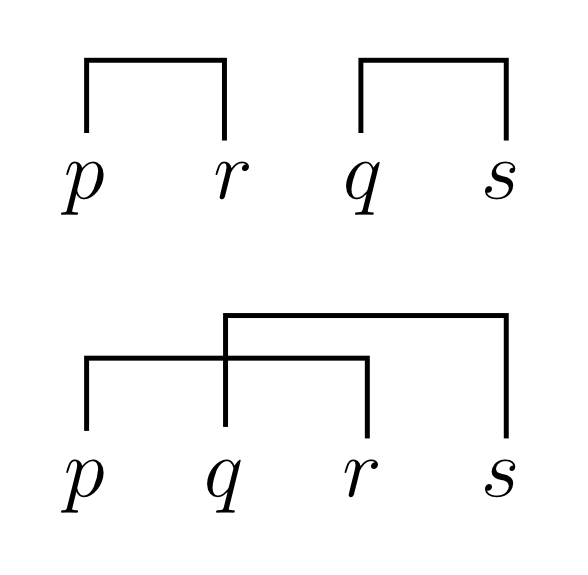
\includegraphics[width=0.4\columnwidth]{figures/determinant_driven/biphasefactor}
		\caption{
		\label{fig:biphasefactor}%
		Crossing of two single excitations
		}
		The third situation doesn't fit the ordering we imposed on excitation operators. $p \leftrightarrow s$ is either lowest electron to highest orbital, or highest electron to lowest orbital.
	\end{center}
\end{figure}

%extra permut si:
%$[(p-r) \oplus (p-s)] \vee [(q-r) \oplus (q-s)] > 0$


% BEGIN Section de TOTO
%----------------------------------------------------------------
\section{Storage of the two-electron integrals}
%----------------------------------------------------------------

In all what follows, all the needed two-electron integrals are kept in memory
and require a fast random access.
A hash table is the natural choice which allows the storage of only non-zero
values with a retrieval of data in nearly constant time, but standard hashing
algorithms tend to shuffle the data to limit the probability of collisions.
Here, we favor instead the locality of the data over the probability of collision
using the hash function given in Algorithm~\ref{alg:hash}.  It returns the same
value for all the keys which are related by the permutation symmetry of the
indices, keeps some locality in the storage of the data, and can be evaluated
in the order of 10 CPU cycles if the integer division by two is replaced by a
bit shift instruction.
\begin{algorithm}[H]
 \caption{HASH}
 \label{alg:hash}
	\SetKwFunction{FMain}{HASH}
	\SetKwProg{Fn}{Function}{:}{}
\Fn(\tcc*[h]{Hash function for two-electron integrals.}){\FMain{$i,j,k,l$}}{
		\KwData{ $i,j,k,l$ are the orbital indices}
		\KwResult{ The corresponding hash .}
        $p \gets \min (i,k)$ \;
        $r \gets \max (i,k)$ \;
        $t \gets p + \frac{1}{2} r (r-1)$ \;
        $q \gets \min (j,l)$ \;
        $s \gets \max (j,l)$ \;
        $u \gets q + \frac{1}{2} s (s-1)$ \;
        $v \gets \min (t,u)$ \;
        $w \gets \max (t,u)$ \;
        \KwRet{$v + \frac{1}{2} w (w-1)$} \;
}
\end{algorithm}

The hash table is such that each bucket can potentially store $2^{15}$
consecutive key-value pairs. The 15 least significant bits of the hash value
are removed to give the index of the bucket ($i_\text{bucket} =
\text{hash}(i,j,k,l)/2^{15}$), and only those 15 bits need to be
stored in the bucket for the storage of the key.
Hence, the storage of the keys only require two bytes per key.
The keys within a bucket are sorted in increasing order, enabling a binary
search to resolve the conflicts. The binary search of the key is always fast
since the binary search is bounded by 15 misses and the maximum size of the
array of keys is 64~kiB, the typical size of the L1 cache.

To accelerate the access to the most frequently used integrals, all the
integrals involving the $128$ closest MOs (molecular orbitals) to the Fermi
level are copied in a dense array of $128^4$ elements ($2$~GiB) enabling a
direct access.

% TODO: Voila les mesures, a mettre dans un tableau

% H2O, cc-pVQZ, 115 MOs
% Array:
%         115 MOs
% Random function :   4.999999950000000E-008
% Random access :   1.299999987000000E-007
% loop ijkl :   6.289285701523365E-009
% loop ikjl :   6.289285701523365E-009
% loop ijlk :   5.717532455930332E-009
% loop lkji :   3.945097394591929E-008
% loop lkij :   3.887922070032626E-008
%Wall time : 4.15901m
% CIPSI : Wall time : 1.54942m

% 
% Map:
% Random function :   4.999999950000000E-008
% Random access :   3.199999968000000E-007
% loop ijkl :   8.233246736539678E-008
% loop ikjl :   1.183529218377579E-007
% loop ijlk :   7.547142841828039E-008
% loop lkji :   8.233246736539678E-008
% loop lkij :   7.547142841828039E-008
%Wall time : 13.4311m
% CIPSI : Wall time : 3.40127m

% END Section de TOTO


\section{generating a subspace}
duplicates are avoided by checking connection to the past \\
******** (ptet exemple avec generator\_CAS versus generator\_full PSI is filtered with different function and supplied to the module using cas\_sd ( cas\_sd, mrcc ) or full\_ci ( pt2 stoch ) )?? \\
================

Generally speaking, a subspace is defined by a reference and a class of excitation applied to it. Because of the determinant-driven approach, it may not be possible to store all the determinants of the considered subspace. 

% - as a matter of fact there is no algorithm to systematically generate all determinants for a defined subspace. The idea to 


\paragraph{reference}

The quantum package allows to define either a CAS or the full-CI as the reference ( although the full-CI is a particular CAS, it is treated differently at the code level ).

\paragraph{excitation class}
The excitations to be applied to the reference are defined by 6 sets of spinorbitals
\begin{itemize}
\item
Holes and particles allowed for single excitations (2 sets)
\item
Holes and particles allowed for the first of a double excitation (2 sets)
\item
Holes and particles allowed for the second of a double excitation (2 sets)
\end{itemize}

This allows to accurately define a subspace. Typically, to define a CAS-SD

\begin{itemize}
\item
\emph{core orbitals} : part of no sets
\item
\emph{inactive orbitals} : part of all "hole" sets
\item
\emph{active orbitals} : part of all sets
\item
\emph{virtual orbitals} : part of all "particle" sets
\item
\emph{deleted orbitals} : part of no set
\end{itemize}


 As will be seen later, determinants are selected iteratively. The general procedure is shown 



\begin{algorithm}
	\caption{GENERAL\_SELECTION}	
	\label{alg:GENERAL_SELECTION}	
	$\ket {\Psi} \gets \ket {HF}$\;
	add CAS spinorbitals to $H_0, H_1, H_2, P_0, P_1, P_2$ \;
	$\hat T$ the list of excitations allowed on the reference based on $H_0, H_1, H_2, P_0, P_1, P_2$ \;
	
	\While{some condition}{
		$C$ the list of determinants of $\Psi$ that are part of the CAS reference \;
		\ForAll{$C_i \in C$}{
			\ForAll{$T_j \in T ; T_j \ket {C_i} \neq 0$}{
				$\ket \alpha \gets T_j \ket {C_i}$ \;
				\If{$not(T_k \ket {C_{l<j}} = \ket \alpha) \&\ Selection\_criterion$}{
					add $\ket \alpha$ to $\Psi '$ \;			
				}
			}
		}
		do some selection in $\Psi'$ \;
		add selected determinants to $\Psi$ \;
		diagonalize $\Psi$ \;
	}
\end{algorithm}

\end{document}
